% RAG pipeline evaluation snippet.
% Required packages: \usepackage{booktabs}, \usepackage{pgfplots}
% Recommended once in the preamble: \pgfplotsset{compat=1.18}

\subsection{Evaluation of the Modular RAG Pipeline}

The evaluation uses the Gherkin requirement dataset stored under
\texttt{requirements/gherkin}. The dataset contains 17 scenarios and 294
Gherkin steps. Each generated Robot Framework keyword call is checked against
the keyword vocabulary extracted from the project's resource files under
\texttt{Resource}. A generated keyword is counted as hallucinated when its
keyword name does not appear in this project resource vocabulary.

The modular RAG pipeline is compared with a zero-shot baseline. The baseline is
implemented as an ungrounded Robot/Selenium-style generator: it converts Gherkin
steps into common generic Robot keyword calls without reading the project
resource catalog, without project-specific preprocessing, and without a
retrieved keyword dictionary in the prompt. This baseline approximates a naive
zero-shot generation setting in which the model relies on generic automation
knowledge instead of the project's existing keyword layer.

\paragraph{Metrics.}
Hallucination Rate (HR) is computed as the percentage of generated keyword calls
whose keyword name is absent from the project resource files. Step Mapping
Accuracy (SMA) is computed as the percentage of scenarios where the number of
generated Robot Framework keyword calls exactly matches the number of source
Gherkin steps. Syntax Errors Count reports generated calls that match a project
keyword name but violate the keyword interface, for example by providing too few
or too many arguments.

\begin{table}[htbp]
\centering
\caption{Comparison of modular RAG and zero-shot baseline on the Gherkin dataset.}
\label{tab:rag_pipeline_evaluation}
\begin{tabular}{lrrrrrr}
\toprule
Pipeline & Source Steps & Generated Keywords & Hallucinated Keywords & HR (\%) & SMA (\%) & Syntax Errors \\
\midrule
Modular RAG & 294 & 294 & 2 & 0.68 & 100.00 & 0 \\
Zero-Shot Baseline & 294 & 373 & 373 & 100.00 & 5.88 & 0 \\
\bottomrule
\end{tabular}
\end{table}

\begin{figure}[htbp]
\centering
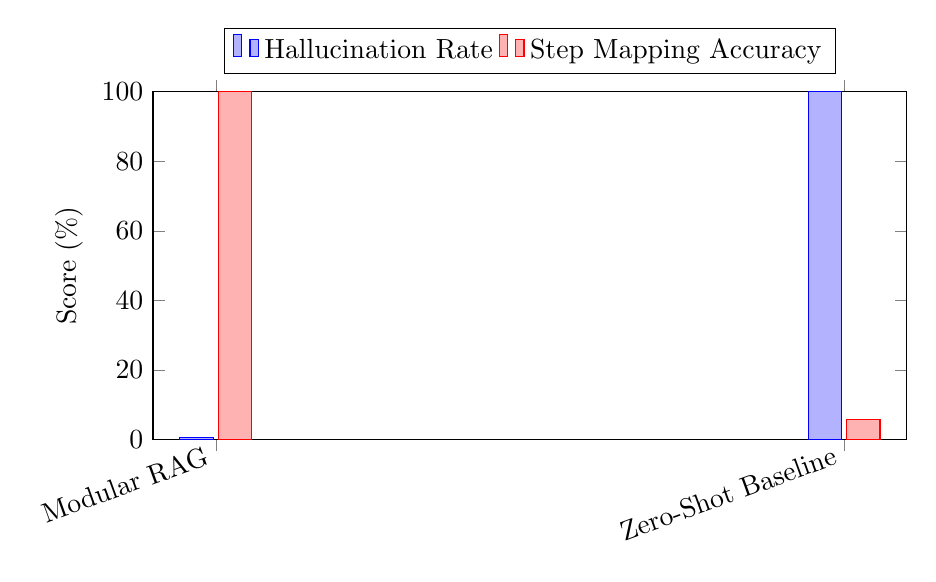
\begin{tikzpicture}
\begin{axis}[
    ybar,
    ymin=0, ymax=100,
    ylabel={Score (\%)},
    symbolic x coords={Modular RAG,Zero-Shot Baseline},
    xtick=data,
    x tick label style={rotate=20, anchor=east},
    bar width=12pt,
    width=0.92\linewidth,
    height=6cm,
    legend style={at={(0.5,1.05)}, anchor=south, legend columns=2},
]
\addplot coordinates {({Modular RAG},0.68) ({Zero-Shot Baseline},100.00)};
\addplot coordinates {({Modular RAG},100.00) ({Zero-Shot Baseline},5.88)};
\legend{Hallucination Rate, Step Mapping Accuracy}
\end{axis}
\end{tikzpicture}
\caption{Hallucination rate and step mapping accuracy for the modular RAG pipeline and the zero-shot baseline.}
\label{fig:rag_pipeline_evaluation}
\end{figure}

The modular RAG pipeline achieves a hallucination rate of 0.68\%, compared with
100.00\% for the zero-shot baseline. The two hallucinated modular outputs are
the fallback keyword \texttt{No Operation} generated for two intentionally
unsupported negative-control steps in \texttt{No\_operation\_test.feature}. The
modular pipeline also preserves one-to-one step alignment for all scenarios
(SMA = 100.00\%), while the zero-shot baseline over-generates generic low-level
commands and only preserves the expected step count in 1 of 17 scenarios
(SMA = 5.88\%).
